

\CLe\ were introduced by Gibbon and McGuinness\rf{GibMcCLE82} as a low-dimensional model
of baroclinic instability in the atmosphere.
As the name suggests they turned out to be a complex generalization
of Lorenz equations:
\beq
\index{Complex Lorenz equations}
\begin{split}
 \dot{x} &=-\sigma x+ \sigma y \,,\\
 \dot{y} &=(r-z)x-a y \,,\\
 \dot{z} &= \frac{1}{2}\left(x \bar{y}+\bar{x}y\right)-b z\,,
 \label{eq:CLe}
\end{split}
\eeq
where now $x,y$ are complex variables, $z$ is real, while the parameters $\sigma,\,b$ are real and $r=r_1+i r_2$, $a=1-i e$ are
complex. In the special case $r_2=0, e\neq0$, \CLe\ also appear as a truncation of Maxwell-Bloch equations describing detuned lasers\rf{BakasovAbraham93}
	\ES{This is were the correspondance is established in a satisfactory manner, while criticising the choice of Ning and Haken\rf{NingHakenCLE90} to
		take $r_2=-e$.}
.
As allready noted \CLf\ is equivariant under the action \refneq{eq:RotCLe} of $\SOn{2}$. 
We rewrite the system in real variables $x=x_1+ i\, x_2\,,\ y=y_1+i\, x_2$ as
\beq
\begin{split}
	\dot{x}_1 &= -\sigma x_1 + \sigma y_1\cont
	\dot{x}_2 &= -\sigma x_2 + \sigma y_2\cont
	\dot{y}_1 &= (r_1-z) x_1 - r_2 x_2 -y_1-e y_2 \cont
	\dot{y}_2 &= r_2 x_1 + (r_1-z) x_2 + e y_1- y_2\cont
	\dot{z} &= -b z + x_1 y_1 + x_2 y_2\,.
	\label{eq:CLeR}
\end{split}
\eeq
The \stabmat\ is
  \beq
{\Mvar_{CLe}} =
  \left(\barr{ccccc}
    -\sigma    	& 0 		& \sigma & 0    &  0 \\
	0 	& -\sigma       & 0      & -\sigma   &  0 \\
	r_1-z  &     -r_2      & -1     & -e & -x_1 \\
	r_2     & r_1-z       	& e  	& -1       & -x_2 \\
	y_1     & y_2           & x_1    & x_2      & -b
    \earr\right)
\,.
  \ee{CLeStabMat}
The origin is a \eqv\ of \refeq{eq:CLeR} for any value of the parameters. As shown in
\refref{FowlerCLE82} it is stable for $0<r_1<r_{1c}$ and unstable for $r_{1c}<r_1$, where
\beq
	r_{1c} = 1 + \frac{(e+r_2)(e-\sigma r_2)}{(\sigma+1)^2}\,.
\eeq
At bifurcation a pair of eigenvalues crosses the imaginary axis with imaginary part:
\beq
	\omega_c = \frac{\sigma (e + r_2)}{\sigma+1}\,.
	\label{eq:omegaCLE}
\eeq

Thus we can expect that after a center manifold or Liapunov-Schmidt reduction one
can apply the equivariant Hopf bifurcation theorem\ES{state it in appropriate section,
refer to it.} with $\SOn{2}$ symmetry
and verify the existence of a \reqv\ after bifurcation\ES{I'll do this
if I have time.}. In \refref{FowlerCLE82} the authors perform a direct bifurcation analysis and
show that, for $e+r_2\neq 0$, a Hopf cycle \REQB{1} is created which also turns out to be an \SOn{2}-orbit,
\ie\ a \reqv. For $e+r_2=0$ the cycle degenerates to an \SOn{2}-orbit of \eqv\ \EQB{1},
since $\omega_c =0$ and the conditions of equivariant Hopf theorem do not apply. 

The secondary bifurcation from the \reqv\ is expected according to Krupa's theorem\ES{refer to it
when written up} to result in relative periodic orbits.
In the non-generic case of an \SOn{2}-orbit of \reqva\
it has been shown by Krupa that one gets bifurcation to periodic orbits. The secondary bifurcation has
been studied in \refref{NingHakenCLE90}.
    \ES{The results are messy and hard to comment on.
They show existence of supercritical and subcritical bifurcations. Will continue this discussion
later}

Ning and Haken\rf{NingHakenCLE90} have shown that certain semiclassical approximations
for single mode, detuned, ring lasers lead to equations isomorphic to \CLe, %with $x,y$ and $z$
%proportional to electric field, polarization and population inversion, respectively.
but the authors choose $e+r_2=0$ so that a detuned stationary solution exists.\ES{This assumption is
questionable unless it is forced by the physics of the problem, which I cannot follow very
well. It leads to non-generic bifurcation behavior, while one would like a model of
a physical system to be robust under perturbations (of the model). Furthermore, the fact that the
Hopf cycle in the general case is an $\SOn{2}$-orbit has gone unnoticed. The \reqv\ can
be interpreted as an \eqv\ in a rotating frame and the measured electric field of the laser
would be the same in both cases.} Bakasov and Abraham\cite{BakasovAbraham93} criticize this approach
and show that one can use \CLe\ with $r_2=0$ and $e\neq0$ to describe detuned lasers. 

\subsection{The $e=r_2=0$ case}

When $e=r_2=0$ we immediately observe the real subspace $x_2=y_2=0$ is flow invariant
and the usual \Le\ are recovered. From equivariance, any subspace $U_\theta$ on the $\SOn{2}$-orbit of the real
subspace is invariant as well, for example the imaginary subspace $x_1=y_1=0$. The
$U_\theta$'s are  parameterized by the angle of \SOn{2} rotations with
the restriction $\theta\in[0,\pi)$. We demonstrate the situation for the standard \Le\ parameters
in \reffig{fig:LorenzCoex}. A continuum of identical, disjoint ``Lorenz mask'' attractors exists.

%%%%%%%%%%%%%%%%%%%%%%%%%%%%%%%%%%%%%%%%%%%%%%%%%%%%%%%%%%%%%%%%%%
\begin{figure}[t]
\begin{center}
  (\textit{a})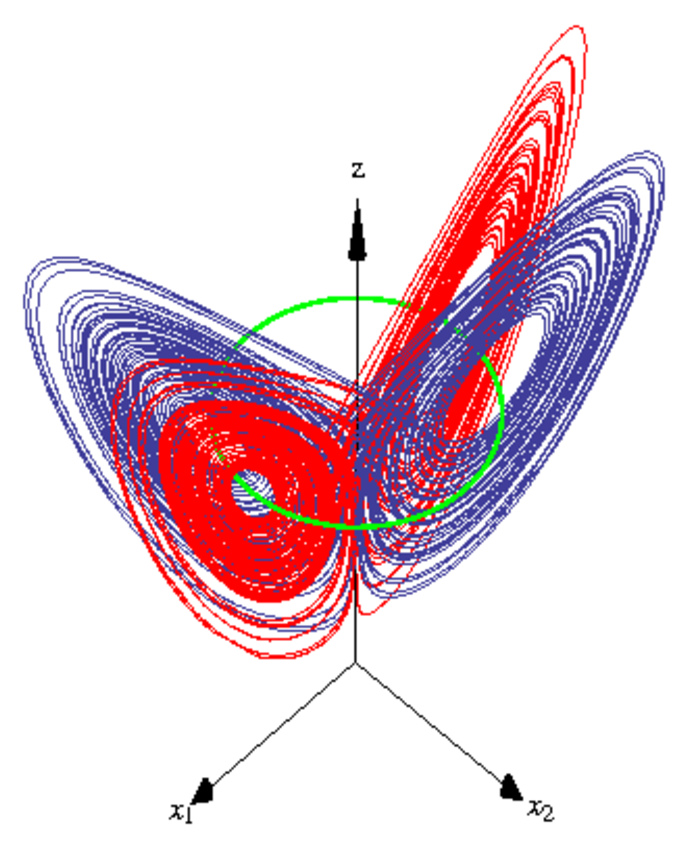
\includegraphics[width=0.35\textwidth]{../figs/LorenzCoexA.eps}
~~~~(\textit{b})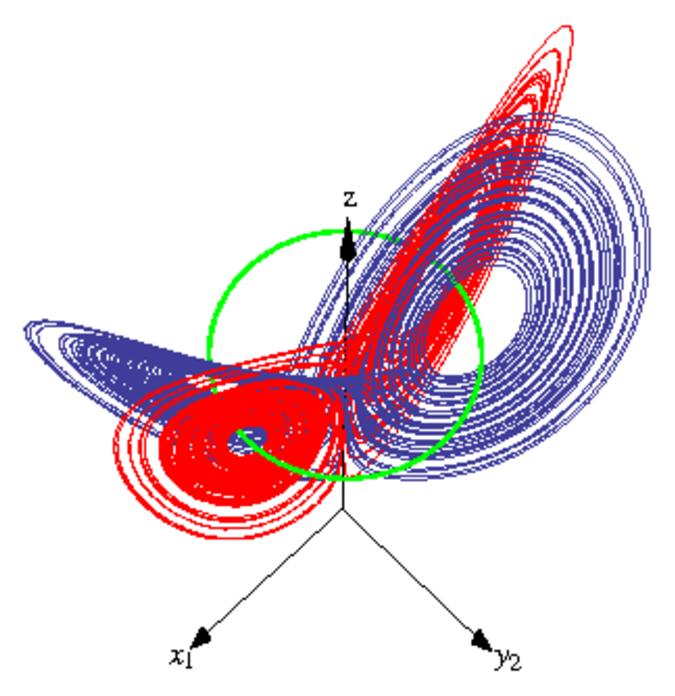
\includegraphics[width=0.35\textwidth]{../figs/LorenzCoexB.eps}
\end{center}
\caption[Complex Lorenz eq. coexisting attractors]{ Two different projections
of the \CLe\ dynamics \refneq{eq:CLe}
for $r_1=28,\, b=8/3,\, \sigma=10,\, a=1$ and $e=r_2=0$. The dynamics in
the real subspace $U_0$ and in $U_{5\pi/6}$ is shown in red, blue respectively. The green circle
is the \SOn{2}-orbit of \eqv\ $E_1$.
    }
\label{fig:LorenzCoex}
\end{figure}
%%%%%%%%%%%%%%%%%%%%%%%%%%%%%%%%%%%%%%%%%%%%%%%%%%%%%%%%%%%%%%%%


Yet, we cannot choose all initial conditions
in one of the flow invariant subspaces $U_\theta$. Indeed, if we use the real subspace
as reference we can choose coordinates $(x_1,y_1,z,\theta)$ for the subspace $U$ of \Rls{5}
foliated by the $U_\theta$'s, which makes it clear that this is a 4-dimensional subspace.
Points that do not lie on $U$ can be thought of as ``mis-rotated'': we start with a point on
the real subspace and rotate by an angle $\theta$ on the $(x_1,x_2)$-plane and by an
angle $\phi\neq\theta$ on the $(y_1,y_2)$ plane. One then would like to know where the asymptotic dynamics
for those initial conditions not in $U$ end up. Since the only \eqva\ of the equations are the origin
and the group orbit of \eqv\ $E_1$, we get the hint that the asymptotic dynamics has to be governed
by the stable and unstable manifolds of the same \eqva\ that govern dynamics in $U$.
To see whether this is true we examine the inner product of the vector field at any point  $a=(x_1,x_2,y_1,y_2,z)$  with the direction of
rotations of the system
% \beq
%   (x_2\ -x_1\ y_2\ -y_1)
%     \left(\barr{c}
% 	 -\sigma x_1 + \sigma y_1 \\
% 	 -\sigma x_2 + \sigma y_2 \\
% 	 (r_1-z) x_1 - r_2 x_2 -y_1-e y_2 \\
% 	 r_2 x_1 + (r_1-z) x_2 + e y_1- y_2\\
% 	 -b z + x_1 y_1 + x_2 y_2\,.
%     \earr\right)
% \,.
% \eeq
\beq
	(\Lg.a).\vf(a) = \left(r_1-\sigma-z\right)\left(x_1 y_2 -x_2 y_1\right) -r_2\left(x_1 y_1+ x_2 y_2\right)- e\left(y_1^2+y_2^2\right)
	\label{eq:CLe0ip}
\eeq
where we have used $\Lg$, the Lie algebra generator of \SOn{2} and $\vf(a)$, the vector field in \refeq{eq:CLeR}.
We observe that for $e=r_2=0$ only $x_1 y_2-x_2 y_1$ and $z$ appear. By taking the time derivative of $x_1 y_2-x_2 y_1$ and using \refeq{eq:CLeR}
we can show that
\beq
	\frac{d}{dt}\left(x_1 y_2-x_2 y_1\right)= -(\sigma+1)\left(x_1 y_2-x_2 y_1\right)
\eeq
and, since $z$ is bounded, the inner product in \refeq{eq:CLe0ip} goes to zero as $t\rightarrow\infty$\footnote{We cannot have $\sigma\leq -1$.}. Thus, asymptotically the vector
field along any trajectory becomes orthogonal to the direction of infinitesimal rotations and the dynamics approach one of the $U_\theta$'s.
This is demonstrated in \reffig{fig:CLe0trans}.

%%%%%%%%%%%%%%%%%%%%%%%%%%%%%%%%%%%%%%%%%%%%%%%%%%%%%%%%%%%%%%%%%%
\begin{figure}[t]
\begin{center}
  (\textit{a})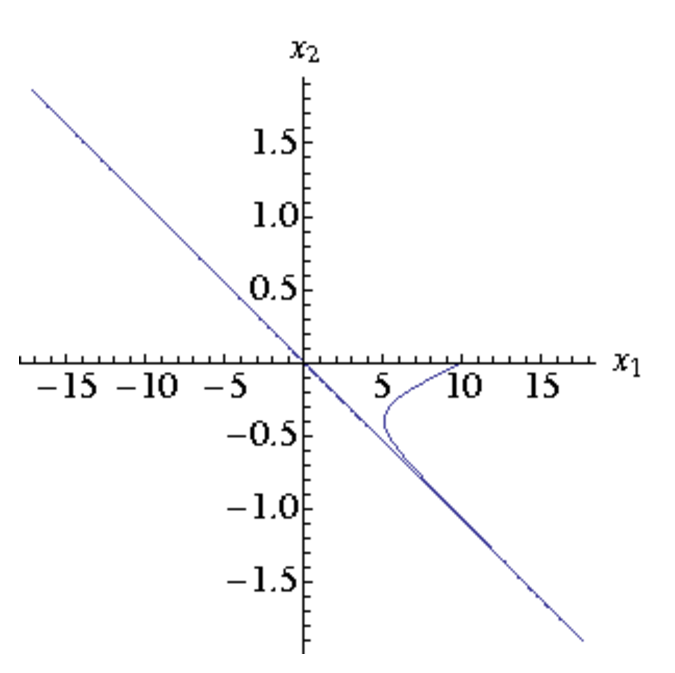
\includegraphics[width=0.35\textwidth]{../figs/CLe0transA.eps}
~~~~(\textit{b})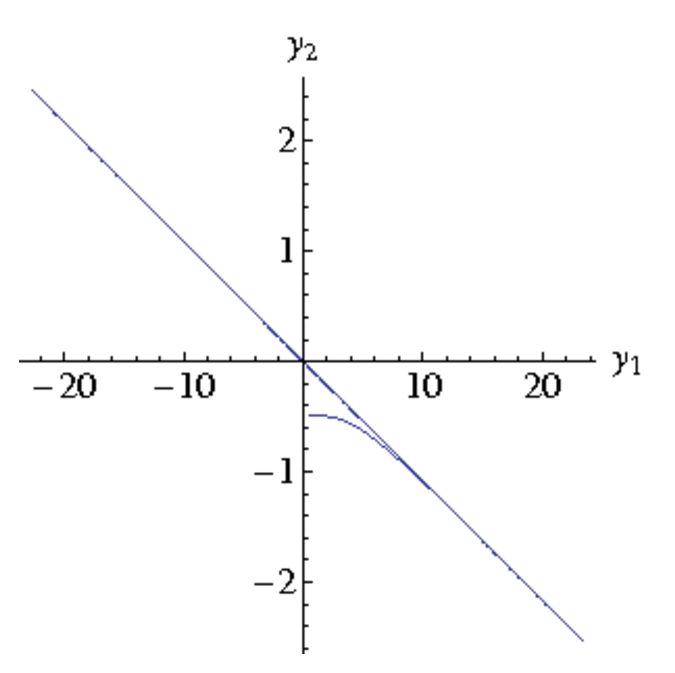
\includegraphics[width=0.35\textwidth]{../figs/CLe0transB.eps}
\end{center}
\caption[Transient trajectory in degenerate Complex Lorenz eq.]{ A trajectory
of the \CLe\ dynamics for $r_1=28,\, b=8/3,\, \sigma=10,\, a=1$ and $e=r_2=0$ with
initial conditions on the complement of $U$ in \Rls{5}. (a) Projection on the
complex $x$-plane, (b) Projection on the complex $y$-plane. The trajectory
approaches some $U_\theta$.
    }
\label{fig:CLe0trans}
\end{figure}
%%%%%%%%%%%%%%%%%%%%%%%%%%%%%%%%%%%%%%%%%%%%%%%%%%%%%%%%%%%%%%%%

\subsection{The $e\neq0,\ r_2=0$ case}

In this section we turn to the ``laser case'' $e\neq0,\ r_2=0$. We work with
parameters $r_1=28,\, b=8/3,\, \sigma=10,\, a=1$ that correspond
to the standard Lorenz values and with detuning set to $e=1/10$.
\refFig{fig:CLE} illustrates the need to project dynamics on \reducedsp: Dynamics
is organized by the interplay of the stable and unstable manifolds of \eqv\ \EQB{0}
and \reqv\ \REQB{1} but the dynamics along the direction of rotation blur the picture
and the notion of recurrence becomes relative. We will present various approaches
to orbit space reduction in the following sections.


%%%%%%%%%%%%%%%%%%%%%%%%%%%%%%%%%%%%%%%%%%%%%%%%%%%%%%%%%%%%%%%%%%
\begin{figure}[ht]
\begin{center}
  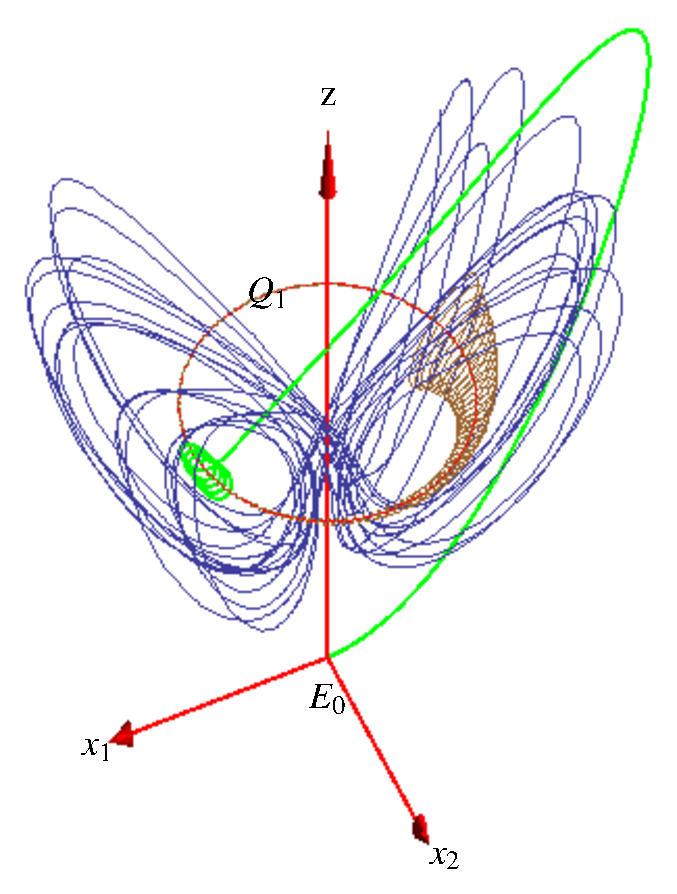
\includegraphics[height=0.25\textheight]{../figs/CLE.eps}
\end{center}
\caption[Complex Lorenz system phase space]{ \Statesp\
portrait of \CLe\ dynamics for $r_1=28,\, b=8/3,\, \sigma=10,\, a=1\, e=1/10,\, r_2=0$.
Plotted are \reqv\ \REQB{1}(red), it's unstable manifold(brown),
\eqv\ \EQB{0}, a representative of it's unstable manifold(green) and a generic orbit(blue).}
\label{fig:CLE}
\end{figure}
%%%%%%%%%%%%%%%%%%%%%%%%%%%%%%%%%%%%%%%%%%%%%%%%%%%%%%%%%%%%%%%%

To find the location of the relative equilibrium it is convenient to work on polar
coordinates defined by $x=\rho_1\phi_1,\,y=\rho_2\phi_2$. Equations \refeq{eq:CLe} with $r_2=0$
take the form
\beq
\begin{split}
	\dot{\rho}_1 &=-\sigma  \rho_1+\sigma \rho_2\cos\Phi \cont
	\dot{\rho}_2 &=-\rho_2 + \rho_1(r_1 -z)\cos\Phi \cont 
	\dot{z} &=  -b z+\rho_1 \rho_2\cos\Phi \cont	
	\dot{\Phi} &=-e-\frac{\sigma \rho_2 \sin\Phi}{\rho_1}+\frac{\rho_1(z-\rho ) \sin\Phi }{\rho_2}\,. 
	\label{eq:CLePolar}
\end{split}
\eeq
where $\Phi=\phi_1-\phi_2$ and the evolution equations for $\phi_1,\phi_2$ are given by
\beq
\begin{split}
	\dot{\phi}_1 &=-\frac{\sigma \rho_2 \sin\Phi}{\rho_1}\cont
	\dot{\phi_2} &= \frac{e \rho_2+\rho_1 (r_1 -z)\sin\Phi}{\rho_2}\,.
	\label{eq:CLeAngl}
\end{split}
\eeq
The condition for a \reqv~ is that all time derivatives in \refeq{eq:CLePolar} vanish from which we get
% Explicit form here, simplified in terms of z component below
% \beq
% \begin{split}
% 	z &= -\frac{e^2}{(\sigma +1)^2}+r_1 -1\cont 
% 	\rho_2 &= \frac{\sqrt{-b \left(e^2+(\sigma +1)^2\right)\left(e^2-(r_1 -1) (\sigma +1)^2\right)}}{(\sigma+1)^2}\cont 
% 	\rho_1 &= \frac{\sqrt{-b \left(e^2-(r_1 -1) (\sigma +1)^2\right)}}{\sigma +1}\cont 
% 	\Phi &= -\cos ^{-1}\left(\frac{\sigma +1}{\sqrt{e^2+(\sigma +1)^2}}\right)
% \end{split}
% \eeq
\beq
\begin{split}
	z^{(1)} &= \frac{-e^2+(r_1 -1)(\sigma +1)^2}{(\sigma +1)^2}\cont 
	\rho_2^{(1)} &= \sqrt{b \left(e^2+(\sigma +1)^2\right)z^{(1)}}\cont 
	\rho_1^{(1)} &= \sqrt{b z^{(1)}}\cont 
	\Phi^{(1)} &= -\cos ^{-1}\left(\frac{\sigma +1}{\sqrt{e^2+(\sigma +1)^2}}\right)
\end{split}
\eeq
Substituting in \refeq{eq:CLeAngl} we get $\dot{\phi}_1=\dot{\phi}_2=e \sigma/(1 + \sigma)\neq 0$ for $e\neq0$
and thus we have indeed a \reqv and not a group orbit of equilibria. 

Calculation  in polar coordinates $\rho_1,\rho_2,\Phi,z$ of stability eigenvalues for \REQB{1} 
for the set of parameters we use here yields 
\beq
	\mu_{1,2}\pm\omega_{1,2}= 0.0938\pm 10.1945i,\, \lambda_3=-11.0009,\, \lambda_4= -13.8534\,.
\eeq



\subsubsection{Invariant Polynomials}


%%%%%%%%%%%%%%%%%%%%%%%%%%%%%%%%%%%%%%%%%%%%%%%%%%%%%%%%%%%%%%%%%%
\begin{figure}[ht]
\begin{center}
  (\textit{a})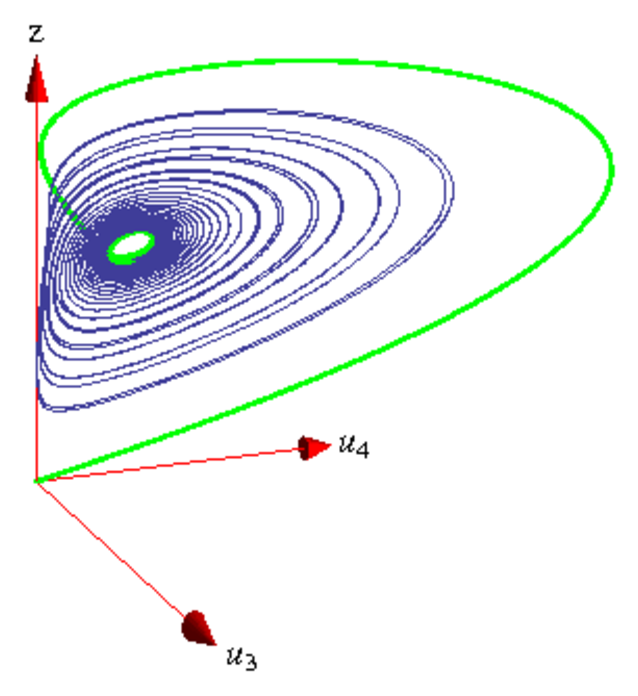
\includegraphics[width=0.35\textwidth]{../figs/CLEip1.eps}
~~~~(\textit{b})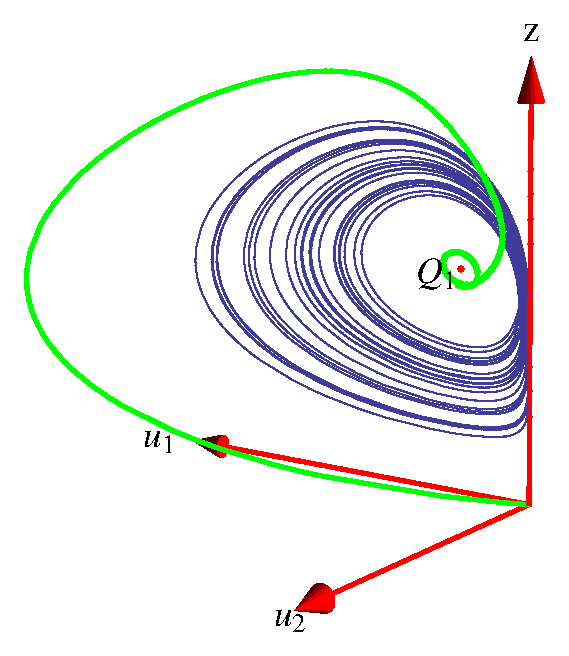
\includegraphics[width=0.36\textwidth]{../figs/CLEip2.eps}
\end{center}
\caption[Orbit space projection of Complex Lorenz system: Invariant polynomials]{ \Statesp\
portraits of \CLe\ dynamics for $r_1=28,\, b=8/3,\, \sigma=10,\, a=1$, $e=1/10$, $r_2=0$
in \reducedsp. Projecting on invariant polynomials \refeq{eq:ipLaser}.
    }
\label{fig:CLEip}
\end{figure}
%%%%%%%%%%%%%%%%%%%%%%%%%%%%%%%%%%%%%%%%%%%%%%%%%%%%%%%%%%%%%%%%

One approach to orbit space reduction is by rewriting the dynamics in
terms of invariant polynomials, following Gilmore and Letellier\rf{GL-Gil07b}:
\beq
\begin{split}
	u_1 &= x_1^2+x_2^2 \cont
	u_2 &= y_1^2+y_2^2 \cont
	u_3 &= x_1 y_2-x_2 y_1\cont
	u_4 &= x_1 y_1+x_2 y_2\cont
	u_5 &= z\,.
	\label{eq:ipLaser}
\end{split}
\eeq
These polynomials are linearly independent, but functionally related by the syzygy
\beq
 	u_1u_2 -u_3^2-u_4^2 =0\,.
	\label{eq:syzLaser}
\eeq
Rather than rewritting the dynamics we merelly map the orbits from original coordinates to $u_i$'s.
Projections of the dynamics on the $u_i$'s are shown in \reffig{fig:CLEip}. In most projections
the folding mechanism is hidden since the dynamics is squeezed near the $z$-axis.
%     \PC{not sure "tearing mechanism" of Gilmore is a good term - noting is
%         torn, it is continuously stretched and then folded with sharp heteroclinic
%         connection edge. {\bf ES:} Agree.}

%%%%%%%%%%%%%%%%%%%%%%%%%%%%%%%%%%%%%%%%%%%%%%%%%%%%%%%%%%%%%%%%%%
\begin{figure}[ht]
\begin{center}
  (\textit{a})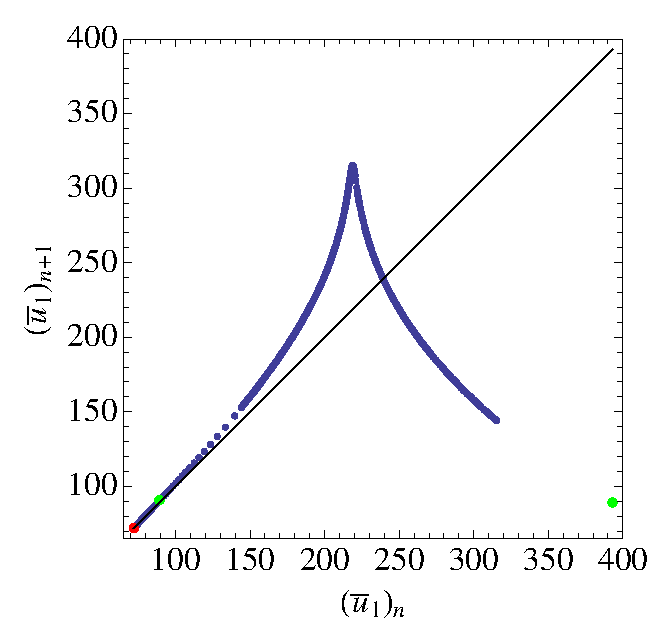
\includegraphics[width=0.35\textwidth]{../figs/CLEipRMu1.eps}
 ~~~~(\textit{b})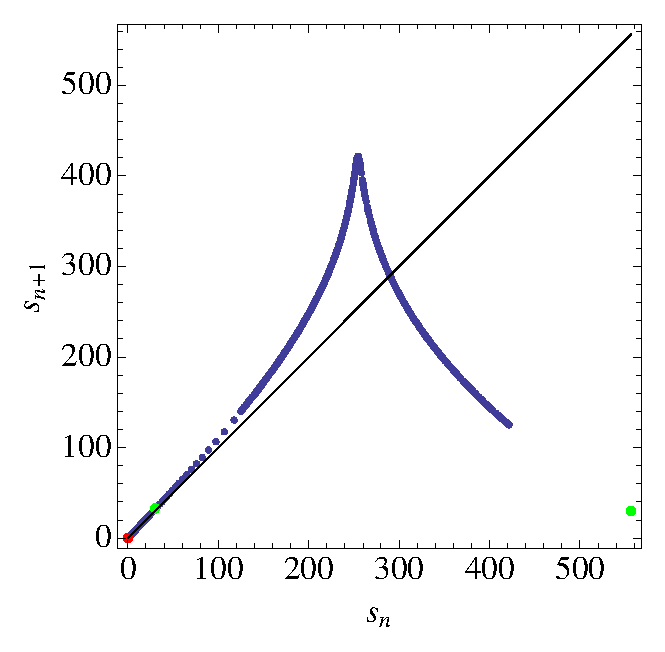
\includegraphics[width=0.35\textwidth]{../figs/CLEipRM.eps}
\end{center}
\caption[\Poincare return map for Complex Lorenz equations, using invariant polynomials]{Return map to the \Poincare
surface of section $u_1=u_4$ for \CLe\ with $r_1=28,\, b=8/3,\, \sigma=10,\, a=1$, $e=1/10$, $r_2=0$,
projecting on invariant polynomials \refneq{eq:ipLaser}. (a) The return map coordinate is
$u_1$, (b) The return map coordinate is the Euclidean
length along the \Poincare cross-section of the unstable manifold of $E_1$.
    }
\label{fig:CLEipRM}
\end{figure}
%%%%%%%%%%%%%%%%%%%%%%%%%%%%%%%%%%%%%%%%%%%%%%%%%%%%%%%%%%%%%%%%

\subsubsection{Moving frame}


%%%%%%%%%%%%%%%%%%%%%%%%%%%%%%%%%%%%%%%%%%%%%%%%%%%%%%%%%%%%%%%%%%
\begin{figure}[ht]
\begin{center}
  (\textit{a})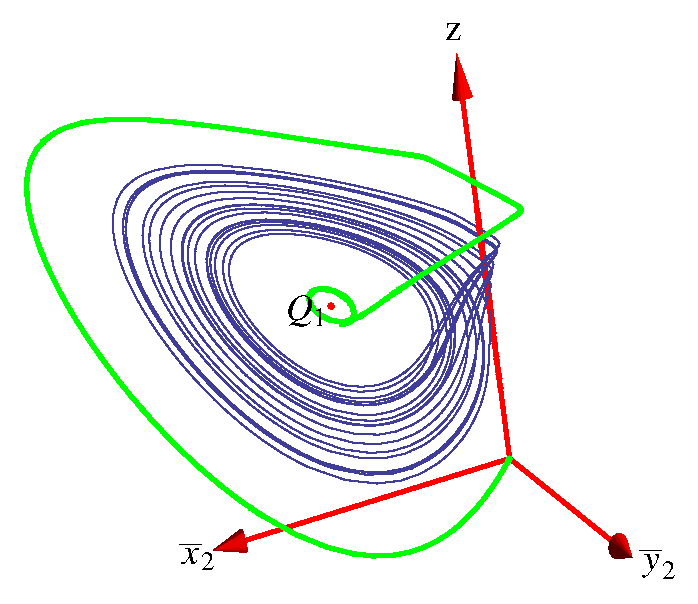
\includegraphics[width=0.35\textwidth]{../figs/CLEmfXYZ.eps}
~~~~(\textit{b})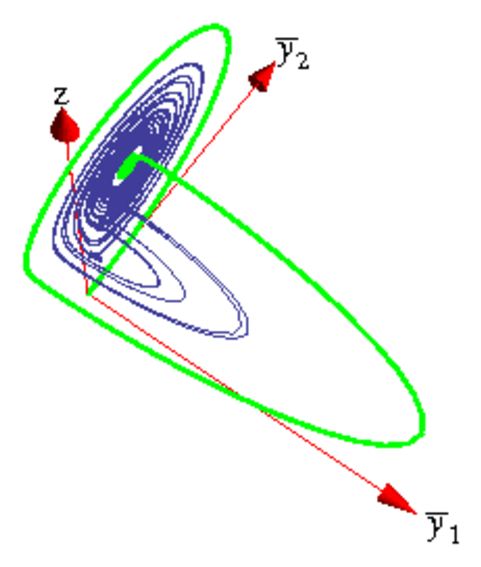
\includegraphics[width=0.35\textwidth]{../figs/CLEmfYYZ.eps}
\end{center}
\caption[Orbit space projection of Complex Lorenz system: Moving frame]{ \Statesp\
portraits of \CLe\ dynamics for $r_1=28,\, b=8/3,\, \sigma=10,\, a=1$, $e=1/10$, $r_2=0$
in \reducedsp. Projecting on invariants given in \refeq{eq:invLaser}.
    }
\label{fig:CLEmf}
\end{figure}
%%%%%%%%%%%%%%%%%%%%%%%%%%%%%%%%%%%%%%%%%%%%%%%%%%%%%%%%%%%%%%%%

As the next choice we explore are the invariants \refneq{eq:invLaser} generated by
the moving frame method that we repeat here for reader convenience:
\beq
\begin{split}
	\theta &= 2 \tan^{-1}\frac{-x_2+\sqrt{x_1^2+x_2^2}}{x_1} \cont
	\overline{x}_2 &= \sqrt{x_1^2+x_2^2} \cont
	\overline{y}_1 &= \frac{x_2 y_1-x_1 y_2}{\sqrt{x_1^2+x_2^2}}\cont
	\overline{y}_2 &=\frac{x_1 y_1+x_2 y_2}{\sqrt{x_1^2+x_2^2}}\,.
	\label{eq:invLaserRepeat}
\end{split}
\eeq

The projections in \reffig{fig:CLEmf} reveal more about the
topology of the attractor but also present large ``jumps." Notice that
the invariants \refneq{eq:invLaser} are related to the invariant polynomials \refneq{eq:ipLaser}
by division by $\sqrt{x_1^2+x_2^2}$ (except the one that is not present.) This is the
reason we get more clear dynamics: All invariants have the same
``dimensions" as the original coordinates. At the same time division by $\sqrt{x_1^2+x_2^2}$
causes the jumps in the $\overline{y}$ components whenever the magnitude of $x$ comes close to zero.
% Notice that we cannot have $x=0$ for dynamics away the $z$-axis due to the syzygy \refneq{eq:syzLaser}. For, if
% $x=0$ then we would also have $y=0$ and thus we would cross the $z$-axis. This cannot happen
% since the $z$ axis is the fixed point subspace of \SOn{2} and is therefore flow-invariant.

Geometrically we can interpret the jumps in the $\overline{y}$ coordinates as follows: We
have chosen to measure angle on one of the irreducible subspaces of \SOn{2}, the $x$-plane, and project
the dynamics on orbit space by counter-rotating in both irreducible subspaces (the $x$- and $y$-plane.)
As long as a trajectory traces one lobe of the Lorenz attractor the angle varies slowly and no
problem occurs. When a trajectory changes quadrant in the $x$-plane to visit the almost opposite lobe (due to detuning
we don't visit the lobe related by rotation by $\pi$, in reality no such thing exists) we get a rapid
change in angle as the trajectory passes close to the origin. In the $y$-plane we don't necessarily change
quadrant. Call $\Delta \theta_x$ and $\Delta\theta_y$ the change in angle
in the $x$- and $y$-plane respectively, when the trajectory changes quadrant in the $x$ plane.
We always reduce to \reducedsp by correcting by $-\Delta\theta_x$ instead of correcting by the smallest angle\ES{I tried
implementing this directly. No luck.}.

% Since $x$ cannot vanish 
The problem is mostly aesthetical in the present case,
but for \KSe\ it will be important to prevent
the denominator from vanishing\ES{Here I have a hunch that the denominator cannot vanish
but I can't prove it}. Since \SOn{2} acts irreducibly in the \CLe\ example
(and also in \KSe) we cannot take more than one irreducible subspace into account
when setting up the normalization equations. We can however restore democracy
between modes by modifying the invariants as follows:
    \PC{replaced ES version
\[\begin{split}
	\overline{x}_2 &= \frac{x_1^2+x_2^2}{\sqrt{x_1^2+x_2^2+y_1^2+y_2^2}} \cont
	\overline{y}_1 &= -\frac{x_2 y_1-x_1 y_2}{\sqrt{x_1^2+x_2^2+y_1^2+y_2^2}}\cont
	\overline{y}_2 &=\frac{x_1 y_1+x_2 y_2}{\sqrt{x_1^2+x_2^2+y_1^2+y_2^2}}\cont
	\overline{z} &=z\,.
	\label{eq:invLaser2}
\end{split}
\]
    }
\beq
\begin{split}
	\overline{x}_2 &= (x_1^2+x_2^2)/r \cont
	\overline{y}_1 &= -(x_2 y_1-x_1 y_2)/r\cont
	\overline{y}_2 &=(x_1 y_1+x_2 y_2)/r\cont
	\overline{z} &=z\cont  
	r &= \sqrt{x_1^2+x_2^2+y_1^2+y_2^2}
    \,.
	\label{eq:invLaser2}
\end{split}
\eeq
This set of invariants lacks a geometric interpretation\ES{or does it?} but results in much cleaner phase portraits,
\cf \reffig{fig:CLEinv}.


%%%%%%%%%%%%%%%%%%%%%%%%%%%%%%%%%%%%%%%%%%%%%%%%%%%%%%%%%%%%%%%%%%
\begin{figure}[ht]
\begin{center}
  (\textit{a})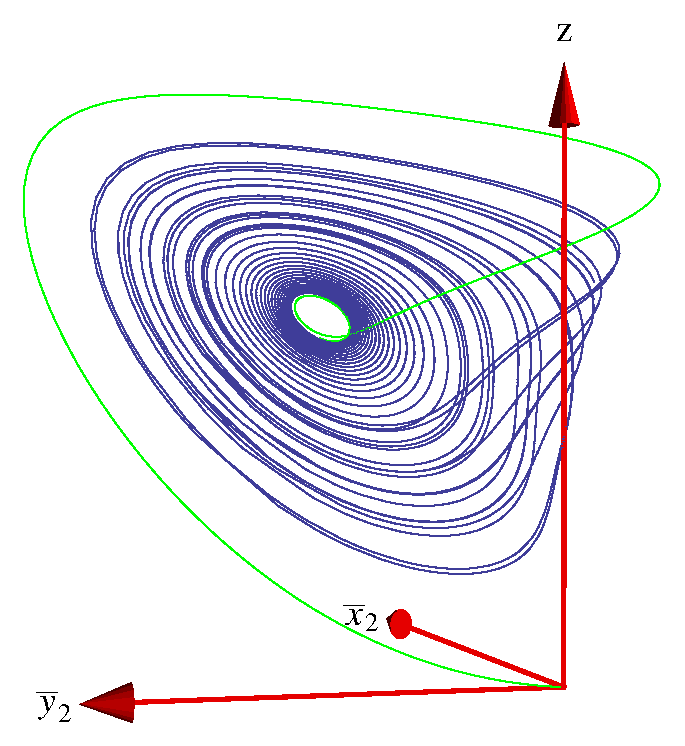
\includegraphics[width=0.35\textwidth]{../figs/CLEinvXYZ.eps}
~~~~(\textit{b})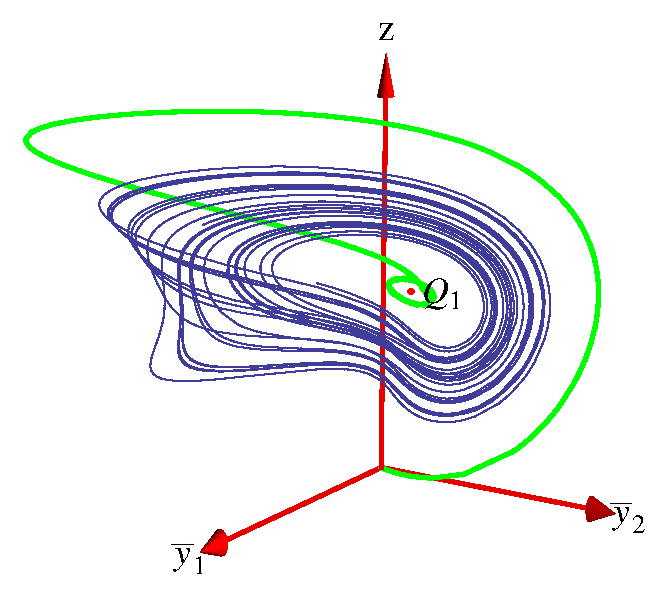
\includegraphics[width=0.35\textwidth]{../figs/CLEinvYYZ.eps}
\end{center}
\caption[Orbit space projection of Complex Lorenz system: Modified moving frame]{ \Statesp\
portraits of \CLe\ dynamics for $r_1=28,\, b=8/3,\, \sigma=10,\, a=1$, $e=1/10$, $r_2=0$
in \reducedsp. Projecting on invariants given in \refeq{eq:invLaser2}.
    }
\label{fig:CLEinv}
\end{figure}
%%%%%%%%%%%%%%%%%%%%%%%%%%%%%%%%%%%%%%%%%%%%%%%%%%%%%%%%%%%%%%%%

%%%%%%%%%%%%%%%%%%%%%%%%%%%%%%%%%%%%%%%%%%%%%%%%%%%%%%%%%%%%%%%%%%
\begin{figure}[ht]
\begin{center}
  (\textit{a})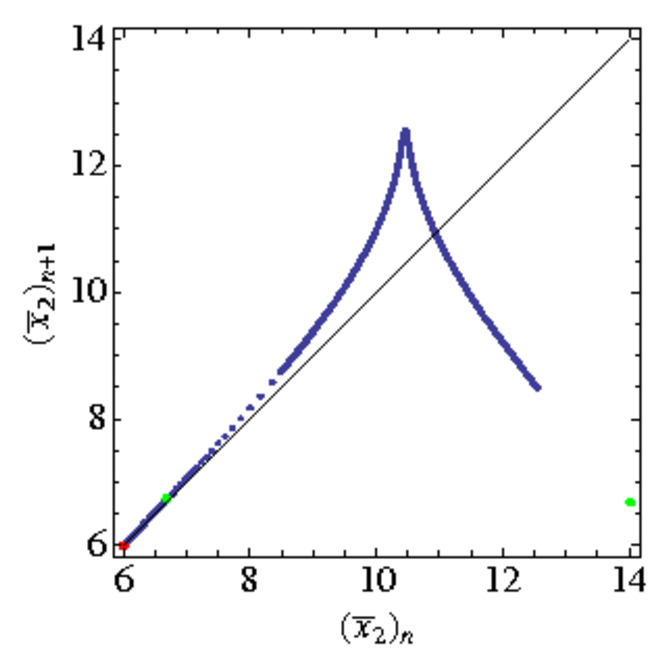
\includegraphics[width=0.35\textwidth]{../figs/CLEinvRMx2.eps}
 ~~~~(\textit{b})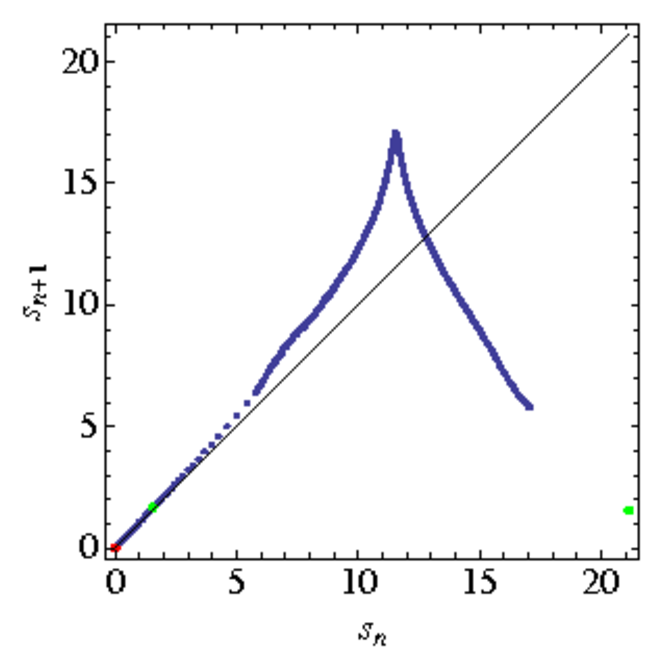
\includegraphics[width=0.35\textwidth]{../figs/CLEinvRM.eps}
\end{center}
\caption[\Poincare return map for Complex Lorenz equations]{Return map to the \Poincare
surface of section $\overline{x}_2=\overline{y}_2$ for \CLe\ with $r_1=28,\, b=8/3,\, \sigma=10,\, a=1$, $e=1/10$, $r_2=0$,
projecting on invariants given in \refeq{eq:invLaser2}. (a) The return map coordinate is
$\overline{x}_2$, (b) The return map coordinate is the Euclidean
length along the \Poincare cross-section of the unstable manifold of $E_1$.
    }
\label{fig:CLEinvRM}
\end{figure}
%%%%%%%%%%%%%%%%%%%%%%%%%%%%%%%%%%%%%%%%%%%%%%%%%%%%%%%%%%%%%%%%


\subsubsection{A geometric approach}

Even though the computation of invariants with the method of the moving coframes is efficient
it is still computationaly prohibitive for high dimensional flows. We will demonstrate
in the example of \CLe\ how one can use the geometric interpretation of the moving coframe method
along with the restriction of the dynamics to a \Poincare section to simply and effectively
perform continuous symmetry reduction in high-dimensional flows.

We have noted that \SOn{2} acts regularly and freely on $X^*=\Rls{5}\backslash\{x_1=x_2=y_1=y_2=0\}$ and
thus we are guaranteed to find the fundamental invariants by the method of moving coframes
if we restrict attention to $X^*$. Nevertheless the transformations \refeq{eq:invLaserRepeat} 
obtained by the moving frame method are singular in the subspace $x_1=x_2=0$\ES{Kevin 
Mitchell claims that what we do here is geometrically impossible because there is
a non-removable singularity isomorphic to the magnetic monopole string singularity. In
this section I argue that we do not do it globally and this is why it is possible (and we
just do it!)}. Therefore
we would like to ensure that we apply our reduction procedure only on points away from this
subspace. A way to achieve this is by a judicious choice of \Poincare section in original space, 
\ie~before reduction. Since we are ultimatelly interested in reducing the dynamics to a \Poincare
return map this is enough for our purposes. Of course locating a \Poincare section is a non-trivial
task on each own right but as we will see in the following, for the procedure to work we will 
have to reduce the candidate \Poincare sections to those that are invariant (as a set) under 
the group action. Furthermore we already have gained the insight from the simpler \Le problem
that a good choice of section is one that passes through the equilibria that organize the flow.
Here we are naturally led to choose a section that passes through the \reqv~\REQB{1} such as the
section $\mathcal{P}_1$ defined by $\overline{x}_2-\overline{y}_2=0$ in the variables of
\refeq{eq:invLaserRepeat} or by $x_1^2+x_2^2-(x_1 y_1 + x_2 y_2)=0$ in original space and
a suitable orientation condition so that trajectories intersect the section away from 
$x_1=x_2=0$ subspace. Here the orientation condition has be chosen so that trajectories intersect
$\mathcal{P}_1$ moving from the ``outside'' of the section in \reffig{fig:CLEmartini} to the 
``inside''. 
Since $\mathcal{P}_1$ has been chosen to be $\SOn{2}$-invariant, the group orbit of any point on
$\mathcal{P}_1$ lies on $\mathcal{P}_1$. In \reffig{fig:CLEmartini} the group orbits of the points
of intersection of \rpo~``01'' have been visualized as circles on $\mathcal{P}_1$. 

The next step is to choose a representative out of each group orbit by means of a section\ES{There is
technical meaning to the word section here.} $\mathcal{P}_2$ that intersects each group orbit
exactly once. The existense of a section is guaranteed since a cross-section as in \refDef{def:cross-section} exists. Here we choose $x_2=0$ for $\mathcal{P}_2$. Geometrically
this is equivalent to rotating each point of intersection on $\mathcal{P}_1$ by
an appropriate angle so that it lies on $\mathcal{P}_2$. This rotation (a linear operation) 
can be applied efficiently even in  high dimensional space when the rotation group acts irreducibly, 
as is frequently the case with truncations of PDE's. Globally the transformation is still non-linear through the dependence on the angle. 


%%%%%%%%%%%%%%%%%%%%%%%%%%%%%%%%%%%%%%%%%%%%%%%%%%%%%%%%%%%%%%%%%%
\begin{figure}[ht]
\begin{center}
  (\textit{a})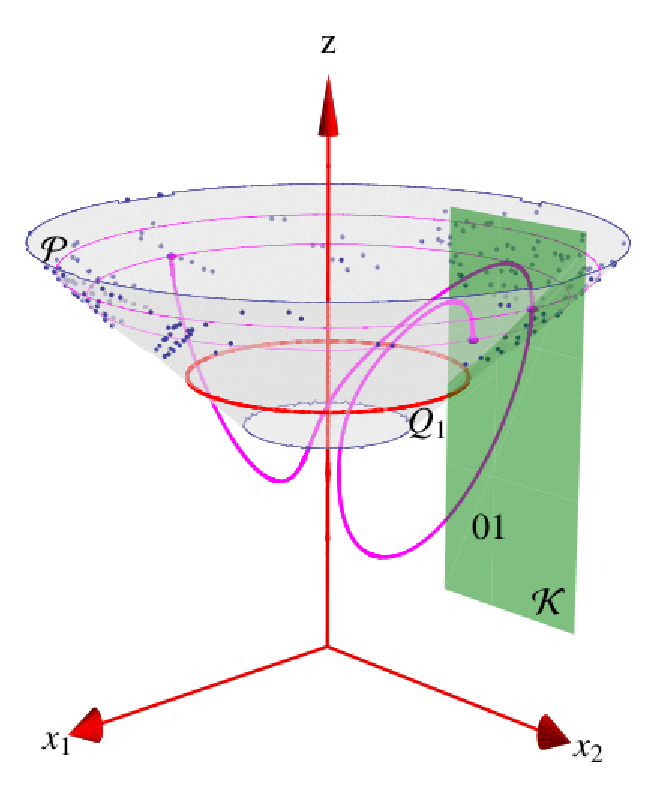
\includegraphics[width=0.35\textwidth]{../figs/CLEmartini.eps}
\end{center}
\caption[\CLe desymmetrization with double section]{Use of \Poincare
surface of section $\mathcal{P}_1$ and section $\mathcal{P}_2$ used for symmetry
reduction of \CLe\ dynamics. 
$\overline{x}_2=\overline{y}_2$ for \CLe\ with $r_1=28,\, b=8/3,\, \sigma=10,\, a=1$, $e=1/10$, $r_2=0$.
Group orbits of the points of intersection of \rpo\ ``01'' have been visualized as circles. 
    }
\label{fig:CLEmartini}
\end{figure}
%%%%%%%%%%%%%%%%%%%%%%%%%%%%%%%%%%%%%%%%%%%%%%%%%%%%%%%%%%%%%%%%